\documentclass[a4paper]{article}
\usepackage[pdftex]{graphicx}
\usepackage[utf8]{inputenc}
\usepackage{enumerate}
\usepackage{icomma}
\usepackage{siunitx}
\sisetup{locale=DE} 
\usepackage{amssymb}
\usepackage{tikz}
\usepackage{href-ul}
\hypersetup{
	colorlinks=true,
	linkcolor=blue,
	urlcolor=blue}
\usepackage{geometry}
\geometry{a4paper, top=15mm, left=15mm, right=15mm, bottom=15mm,
	headsep=10mm, footskip=12mm}

\begin{document}
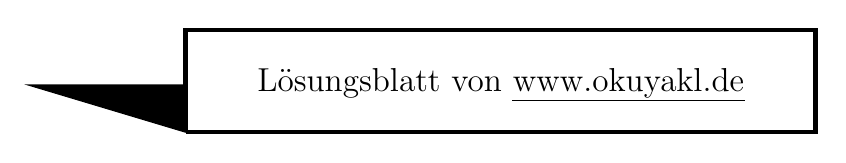
\begin{tikzpicture}(10,3)
	\draw[ultra thick](2,0) --(10,0) -- (10,1.3) --(2,1.3) -- (2,0);
	\draw[fill=black](2,0)-- (0,.6) -- (2,.6) -- (2,0);
	\node at (6,.6) {\large Lösungsblatt von \href{https://www.okuyakl.de}{www.okuyakl.de}};
\end{tikzpicture}
\vspace{0.5 cm}

\noindent
\begin{minipage}{0.5\textwidth}
	\noindent{\bf Aufgabe 1. a)}\\
		\includegraphics[width=7 cm]{gsdrei041}
\end{minipage}
\hfill
\begin{minipage}{0.5\textwidth}
	\noindent{\bf Aufgabe 1. b)}\\
 Das Dreieck ist gleichschenklig, wenn gilt: $\overline{AC}=\overline{BC}$
$$
\renewcommand{\arraystretch}{2}
\begin{array}{rcll}
\sqrt{(7-1)^2 + (4-1)^2} &=& \sqrt{(7-10)^2+(4+2)^2} \\
\sqrt{6^2 + 3^2} &=& \sqrt {3^2+6^2} &(w)\\
\end{array}
$$
\end{minipage}

\noindent{\bf Aufgabe 1. c)}\\
Zuerst berechnet man die  Mittelpunkte zweier Dreiecksseiten.
Durch diese legen wir zwei zu der jeweiligen Seite senkrechte Geraden fest.
Beide Geradenterme setzten wir gleich und erhalten den Schnittpunkt $M$. Dieser ist der Umkreismittelpunkt.

\noindent{\bf Aufgabe 1. d)}\\
Wir betrachten die Streckenlänge $\overline{MA}$:
$$r = \overline{MA}= \sqrt{(5,5-1)^2 + (-0,5-1)^2}=\sqrt{4,5^2 + 1,5^2}=4,74~{\rm LE}$$

\noindent{\bf Aufgabe 1. e)}\\
Der Flächeninhalt des Dreiecks ist:
$$ A_D = {1 \over 2}\cdot \left| \begin{array}{cc} 6 & -3 \\ 3 & 6 \end{array} \right|= {1 \over 2} \cdot (36 + 9) = 22,5~{\rm FE}$$
Der Flächeninhalt des Umkreises ist:
$$A_k = \pi \cdot r^2 = \pi \cdot 4,74^2 = 70,7~{\rm FE} $$
Der Faktor ist :
$$ a = {70,7 \over 22,5}=3,14 = \pi $$

\noindent{\bf Aufgabe 2.}\\
\begin{enumerate}[a)]
	\item falsch, dann ist $0<k<1$
	\item richtig
	\item richtig
	\item falsch, denn sie ist nur winkel- nicht aber längentreu.
\end{enumerate}

\noindent
\begin{minipage}{0.5\textwidth}
	\noindent{\bf Aufgabe 3. a)}\\
	\includegraphics[width=7 cm]{zeg041}
\end{minipage}
\hfill
\begin{minipage}{0.5\textwidth}
	\noindent{\bf Aufgabe 3. b)}\\
	$$\overline{ZP'}= k \cdot \overline{ZP} = 3 \cdot 1,5 = 4,5~{\rm LE}$$
	\noindent{\bf Aufgabe 3. c)}\\
    Die Geradensteigung bleibt bei einer zentrischen Streckung unverändert,
    wir setzen den Punkt $P'(2|6,5)$ in die allgemeine Form ein und erhalten:
    $$
    \renewcommand{\arraystretch}{2}
    \begin{array}{rcll}
    y &=& mx +t \\
    6,5 &=& 0,75\cdot 2 + t \\
     t &=& 5 &\Rightarrow \quad y'=0,75x+5
    \end{array}
    $$
\end{minipage}

\noindent{\bf Aufgabe 3. d)}\\
Es ist ein gleichschenklig-rechtwinkliges Dreieck; sein Flächeninhalt ist:
$$A = {1\over 2} \cdot \overline{AC} \cdot \overline{BC}= {1\over 2} \cdot 2,5^2 = 3,125~{\rm FE}$$

\noindent{\bf Aufgabe 3. e)}\\
Der neue Flächeninhalt ist $k^2$-mal so groß wie der ursprüngliche, also:
$$A'= (-2)^2 \cdot 3,125 = 12,5~{\rm FE}$$

\noindent{\bf Aufgabe 4.}\\
Wenn die Grundfläche $a_U^2$ das Neunfache der Deckfläche $a_O^2$ beträgt, dann gilt für das Verhältnis von Grundkante $a_U$ und oberer Flächenkante $a_O$:
$$
\renewcommand{\arraystretch}{2}
\begin{array}{rcll}
a_U^2 & = & 9 \cdot a_O^2 &| \sqrt{\qquad}\\
a_U   & = & \sqrt{9} \cdot a_O & | : a_O \\
{a_U \over a_O} & = & 3 
\end{array}
$$
Die Höhe der bis zur Spitze ergänzten Pyramide
sei $h_O$, die des Stumpfes sei $h_U=\SI{6}{\centi\meter}$ 
Nach dem Vierstreckensatz gilt dann:
$$
\renewcommand{\arraystretch}{2}
\begin{array}{rcll}
{h_O + h_U \over h_O}& = & {a_U \over a_O} \\
{h_O + h_U \over h_O}& = & 3 & | \cdot h_O \\
h_O + h_U & = & 3 \cdot h_O &| - h_O \\
h_U      & = & h_O\cdot ( 3 - 1) & | :(2)\\
{h_U \over 2} & = & h_O \\
h_O &=& {\SI{6}{\centi\meter} \over 2 } &= \SI{3}{\centi\meter}
\end{array}
$$
Damit ist die Höhe der Spitze über der Grundfläche:
$$h_{ges}=h_U+h_O=\SI{9}{\centi\meter}$$

\begin{center}
	\includegraphics[width=7 cm]{../../viecher/endcomic.pdf}
	
	Hier geht es zurück zum \href{https://www.okuyakl.de/math/m9zesL041/aa041.pdf}{Aufgabenblatt}
\end{center}

\end{document}

